
\chapter{Appendix A - Setting up Google cloud}
\label{ap_gcloud}
There are several cloud services that provides GPU processing, and cloud computing, some of the most popular are Amazon AWS, Microsoft Azure and Google Cloud. These cloud services makes it possible to run code on customisable hardware, and they provide libraries and documentation that makes it easy to set up. In this project Google Cloud was chosen because it gives you 300 USD worth of credit when you open an account, which makes it possible to get to know the framework before you have to pay. That being said, the code being used in this project should be able to run on cloud services by other providers as well. This appendix explains how you set up an account on Google cloud, how you create an instance with the correct hardware, and how one can access a Google Cloud instance from the command line on your own computer. 

\section{Creating an account}
Go to \url{cloud.google.com} and sign in using a Google account. Press "try free", and fill out the form. This will set up a project called "My first project"

\section{Setting up an instance}
After setting up your account, go to the navigation menu in the top left corner, and go to compute engine. Go to VM instances and press create instance. Your screen should look like figure \ref{fig:create_instance1}.

\begin{figure}
    \centering
    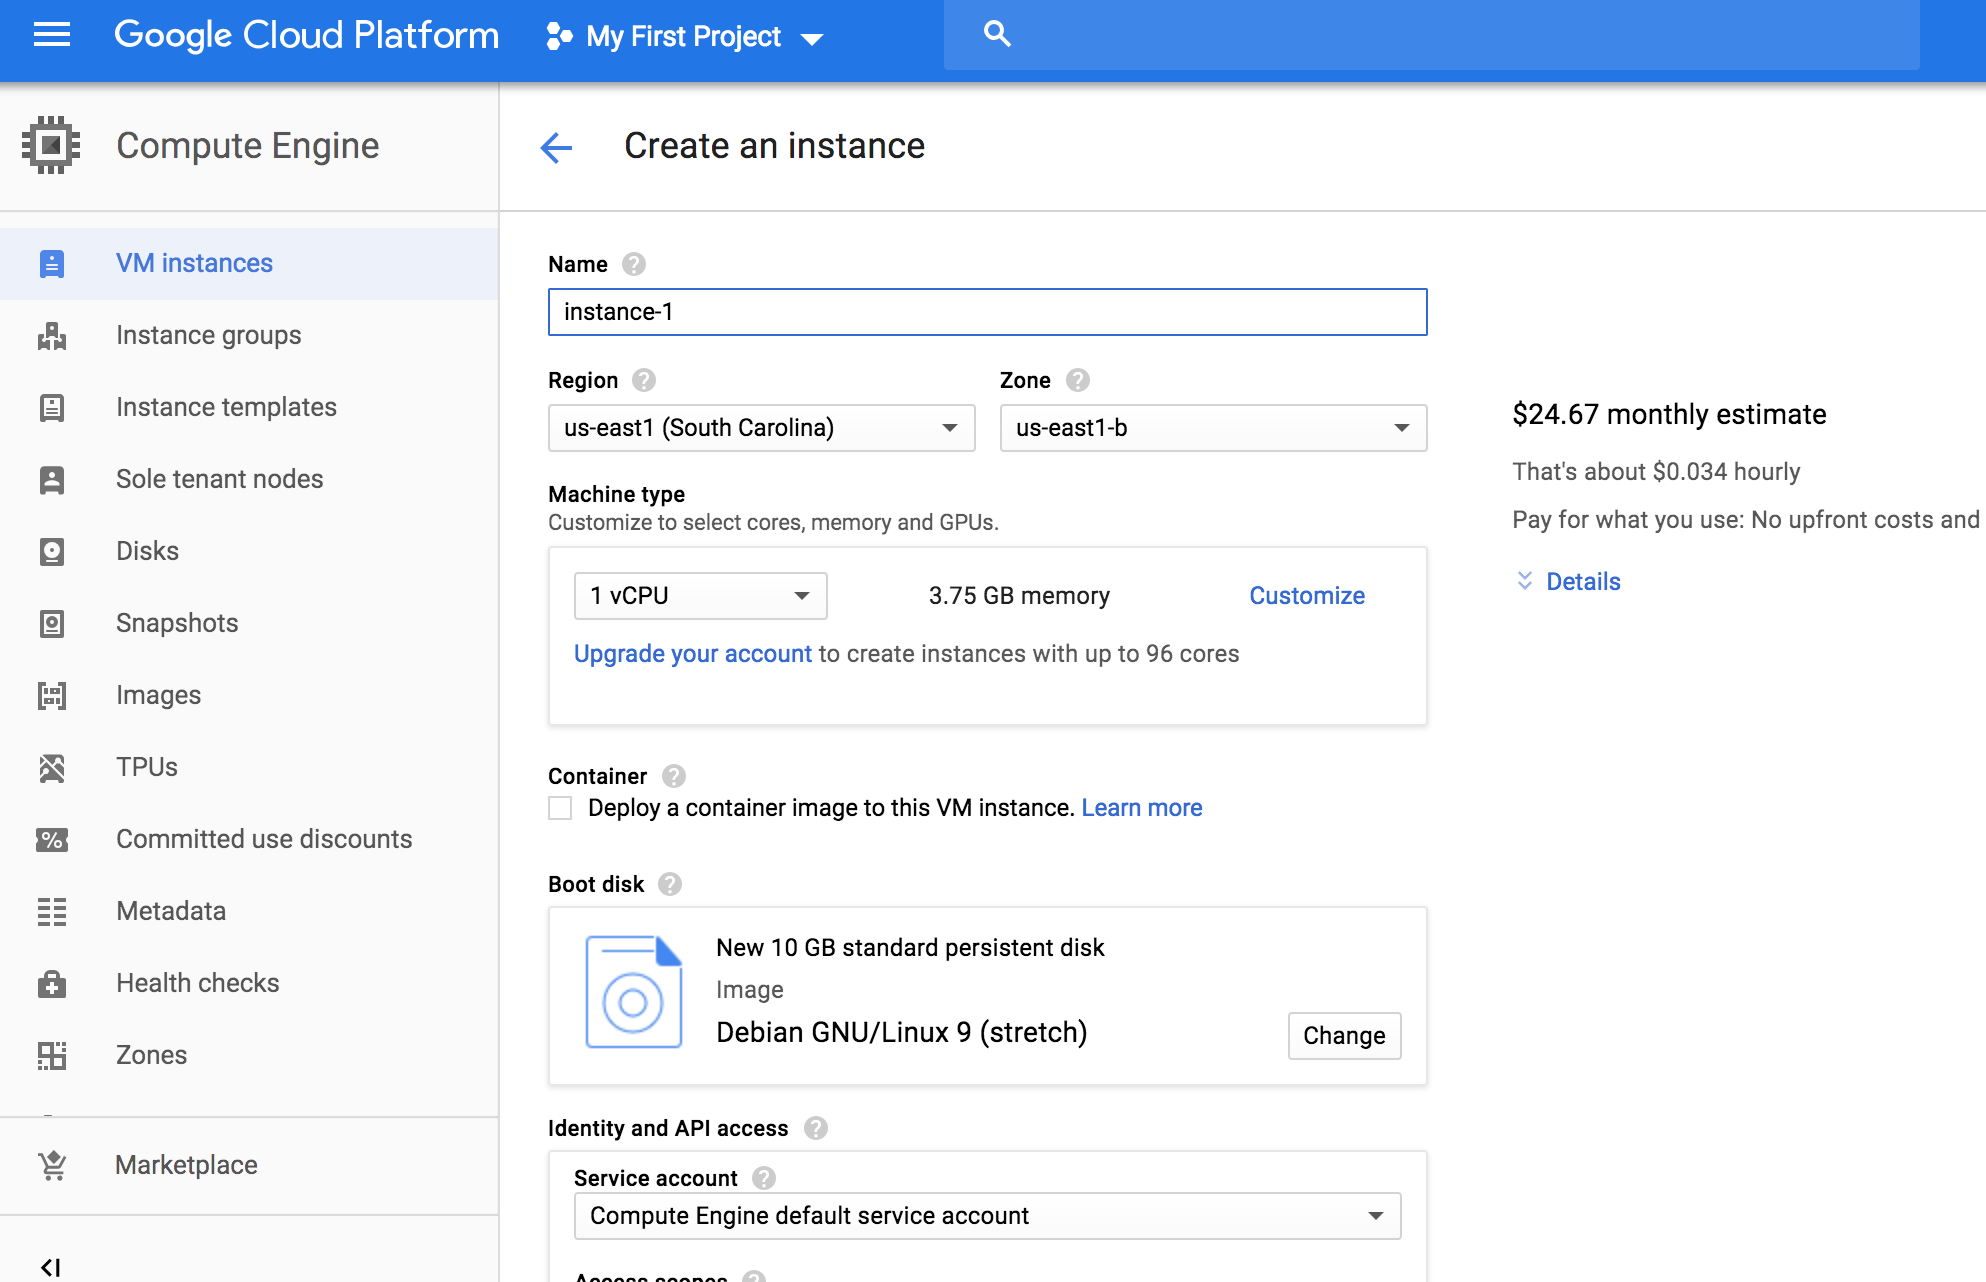
\includegraphics[scale=0.35]{images/create_instance1.png}
    \caption{Create instance}
    \label{fig:create_instance1}
\end{figure}

\newpage
A configuration that has been tested to work is shown in figure \ref{fig:gcloud2}. Here the "Machine type" has been configured with one Nvidia Tesla K80 GPU. Boot disk has been set to Ubuntu 16.04 LTS, and http traffic is allowed. In this example the region is set to "europe-west1(Belgium)", and the zone to "europe-west1-b". The region and zone will affect the hourly price, and some zones and regions does not provide GPUs. There might be different combinations that serves other projects better than the combination chosen in this project. Also the size of the hard drive has been changed from its default value of 10 GB to 100 GB. Which might be necessary when uploading data to the instance. 

\begin{figure}
    \centering
    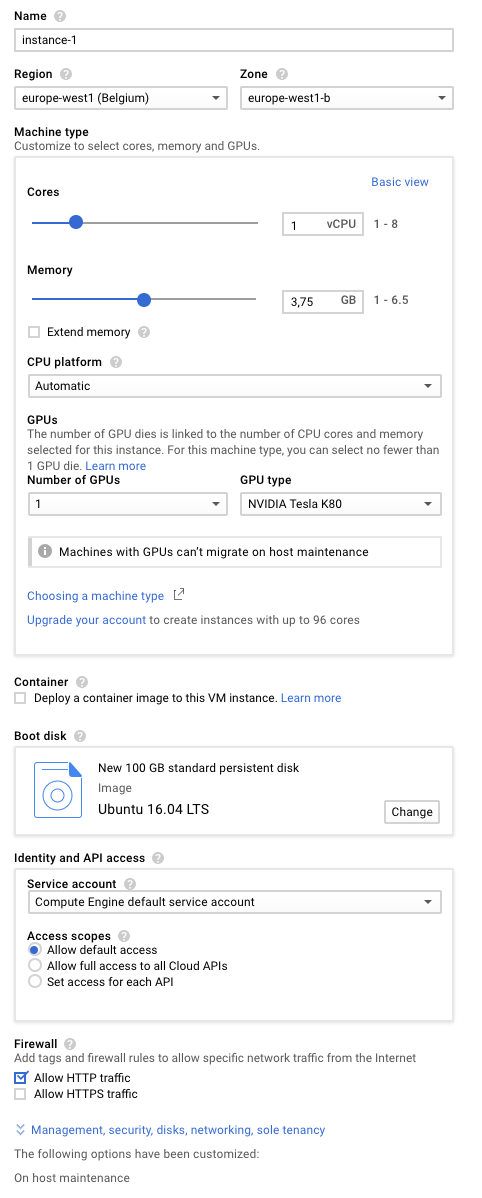
\includegraphics[scale=0.9]{images/gcloud_2.png}
    \caption{Tested configuration}
    \label{fig:gcloud2}
\end{figure}

Press "create instance" and the site will be directed to figure \ref{fig:created_instance}. The green symbol indicates that the instance is running.

\begin{figure}
    \centering
    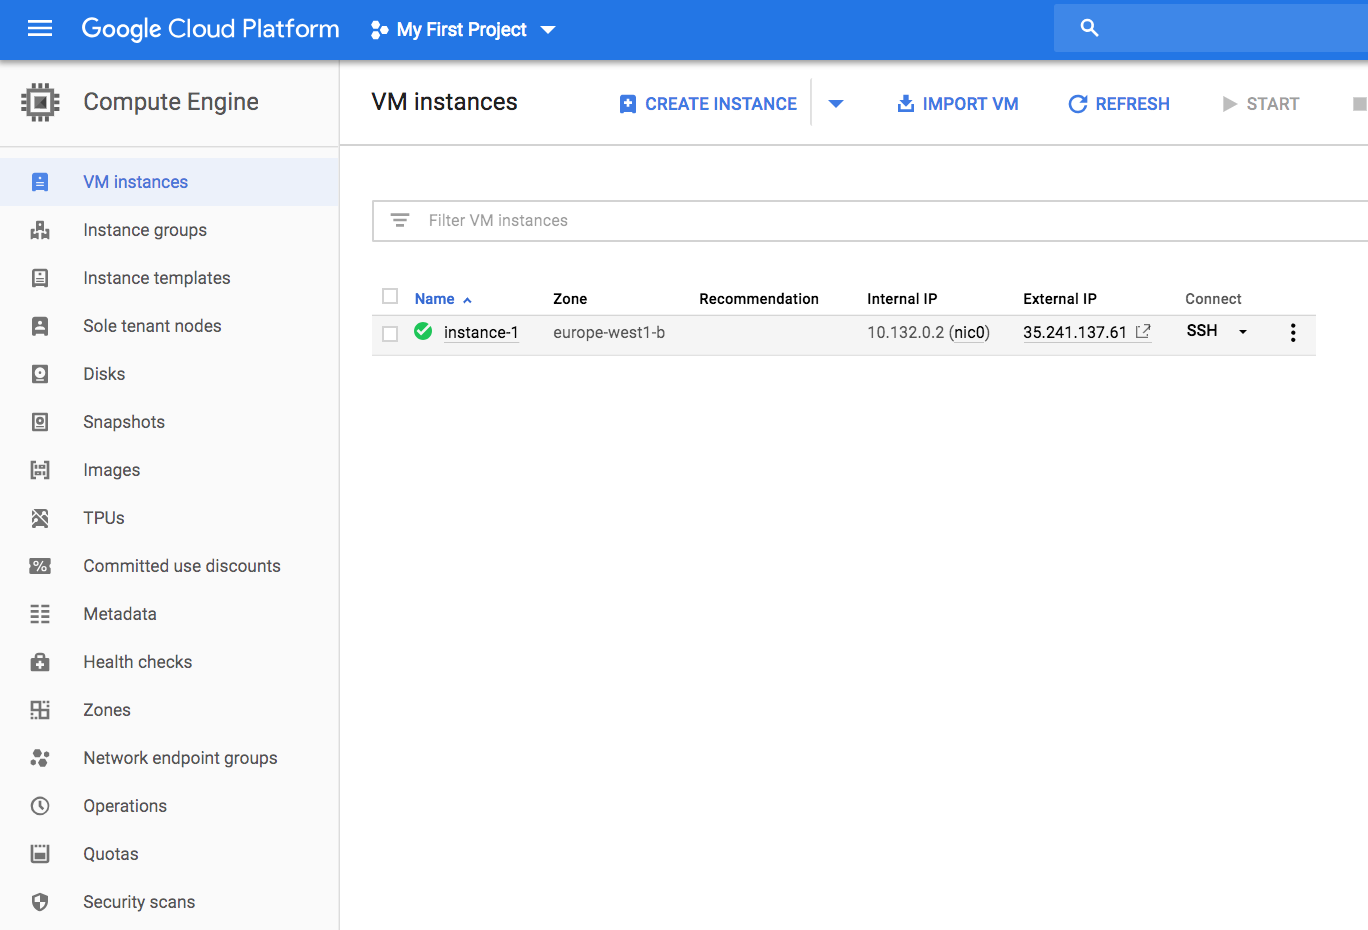
\includegraphics[scale=0.5]{images/created_instance.png}
    \caption{Created instance}
    \label{fig:created_instance}
\end{figure}
\newpage

\section{Setting up  and using gcloud command line tool on local computer}

Install guides for all supported systems can be found on \url{cloud.google.com/sdk/docs/quickstarts}. This guide will take you through the installation process and the initialization process. The initialization process connects the gcloud command line tool to your google cloud account, and lets you access your instances easily when set up correctly. You will be prompted to log in to your Google account, choose project and default zone. Project can be chosen to be the on Gcloud set up when creating your account, and will be the only choice if you did not create new projects. The default zone can be chosen based on your own preference, in this project "europe-west1-b" was used. 

\section{Accessing an instance from local computer using Gcloud command line tool}

When the gcloud command line tool is installed and set up correctly, it can be used to access your instance. The way it has been accessed in this project is through SSH, and with SCP to transfer files. 

\vspace{3mm}
\subsection{SSH in to instance}
To SSH into an instance the following command can be used. <name> and <zone> should be the name and zone of your created instance, as shown in figure \ref{fig:created_instance}.

\begin{lcverbatim}
    gcloud compute ssh <name> --zone <zone>
\end{lcverbatim}
\begin{lcverbatim}
    gcloud compute ssh instance-1 --zone europe-west1-b
\end{lcverbatim}

\subsection{SCP file to instance}
To transfer files to an instance the following command can be used. 
\begin{lcverbatim}
gcloud compute scp <path/to/local/file> \\ 
<name>:/path/to/remote/file --zone <zone>
\end{lcverbatim}
\begin{lcverbatim}
gcloud compute scp /home/data/image.jpg  \\
instance-1:/home/images --zone europe-west1-b
\end{lcverbatim}

This command will transfer the file image.jpg to the images repository on the cloud instance.

\subsection{SCP repository to instance}

\vspace{3mm}
To transfer repositories and their content the following command can be used

\begin{lcverbatim}
gcloud compute scp --recurse </path/to/local/repo> \\ 
<name>:</path/to/remote/repo --zone <zone>
\end{lcverbatim}

\begin{lcverbatim}
gcloud compute scp --recurse /home/data instance-1:/home/ \\ 
--zone europe-west1-b
\end{lcverbatim}
\vspace{3mm}

This command will transfer the "data" repository and its content to the home directory of the instance.




\chapter{Appendix B - Using cloud\_detection\_framework}
After accessing an instance with SSH, the instance can be set up using the Github repository cloud-detection-framework. 

\begin{lcverbatim}
git clone https://github.com/simenvg/cloud\_detection\_framework
\end{lcverbatim}

When the github repository has been cloned, run setup.sh with the following command from your root directory.

\begin{lcverbatim}
./cloud\_detection\_framework/setup.sh
\end{lcverbatim}

This will install CUDA, cudnn, tensorflow and other necessary libraries correctly, build darknet and set up an environment for training and testing both YOLOv3 and SSD. The setup file will run for approximately 10-15 minutes. There exists other releases of the libraries installed, that might be advantageous for other projects. The versions chosen here, are chosen because they are compatible with the hardware used, and work for both the SSD and YOLO implementation. There is no guarantee that anything will work, even after the smallest changes to this file or the hardware of the instance, as I have painfully 

\section{Training}
Both YOLO and SSD uses pretrained weights, this framework makes it possible to further train the networks on a custom dataset. The data can be uploaded to the cloud instance using SCP. 
\newpage
\subsection{Adding datasets and directory structure setup}
In the cloud instance the following directory structure should be used for datasets


\dirtree{%
.1 root.
.2 data.
.3 dataset1.
.4 test.
.5 img1.jpg.
.5 img1.xml.
.4 train.
.5 img2.jpg.
.5 img2.xml.
.3 dataset2.
.3 dataset3.
}

When adding a new dataset, it should be labelled using the VOC format annotation. This can be done using labelImg, from \url{https://github.com/tzutalin/labelImg}. This will produce an xml file for each jpg file labelled, with the same name. Put all the xml and jpg files in the same folder, and run the file split\_dataset.py on the folder by running the following command.

\begin{lcverbatim}
python split_dataset.py /path/to/dataset
\end{lcverbatim}




\subsection{Training YOLO}
To train Yolo, run the file train.py in cloud-detection-framework. To run this file you need to provide the path to darknet, and the path to your data directory.

\begin{lcverbatim}
python train.py /home/user/darknet /home/user/data
\end{lcverbatim}

This file will ask the user which datasets in the data directory Yolo should be trained on, and begin training. 

\subsection{Training SSD}
To train SSD two files need to be run. The first one being convert\_tfrecords.py, and the second being


\chapter{Appendix C}
This appendix contains example images referenced in the thesis.


\newpage

\section{SSD2 and SSD3 on bc bf}
\label{sec:bigbox}

\begin{figure}[h!]
\begin{subfigure}{.5\textwidth}
  \centering
  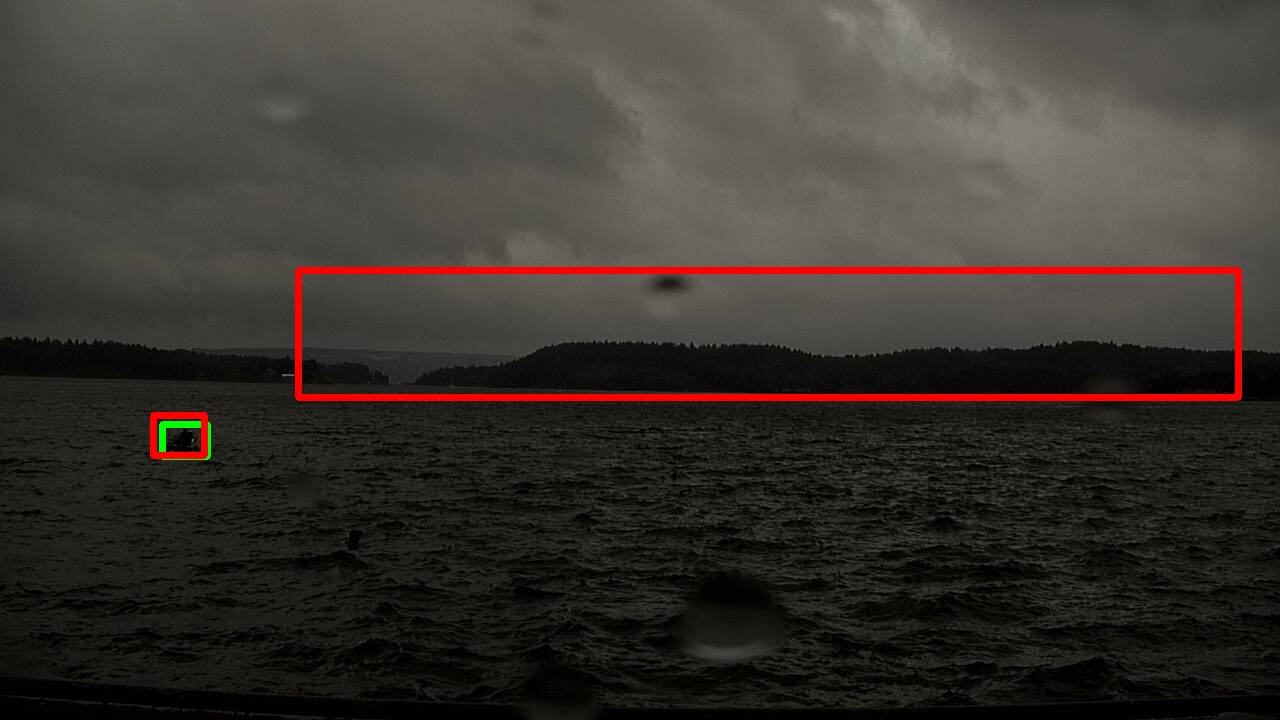
\includegraphics[width=0.9\linewidth]{results/case_buildings/bigbox_bcbf/SSD2/selected_06_14_axis0049.jpg}
  \caption{SSD2}
  \label{fig:sfig1}
\end{subfigure}%
\begin{subfigure}{.5\textwidth}
  \centering
  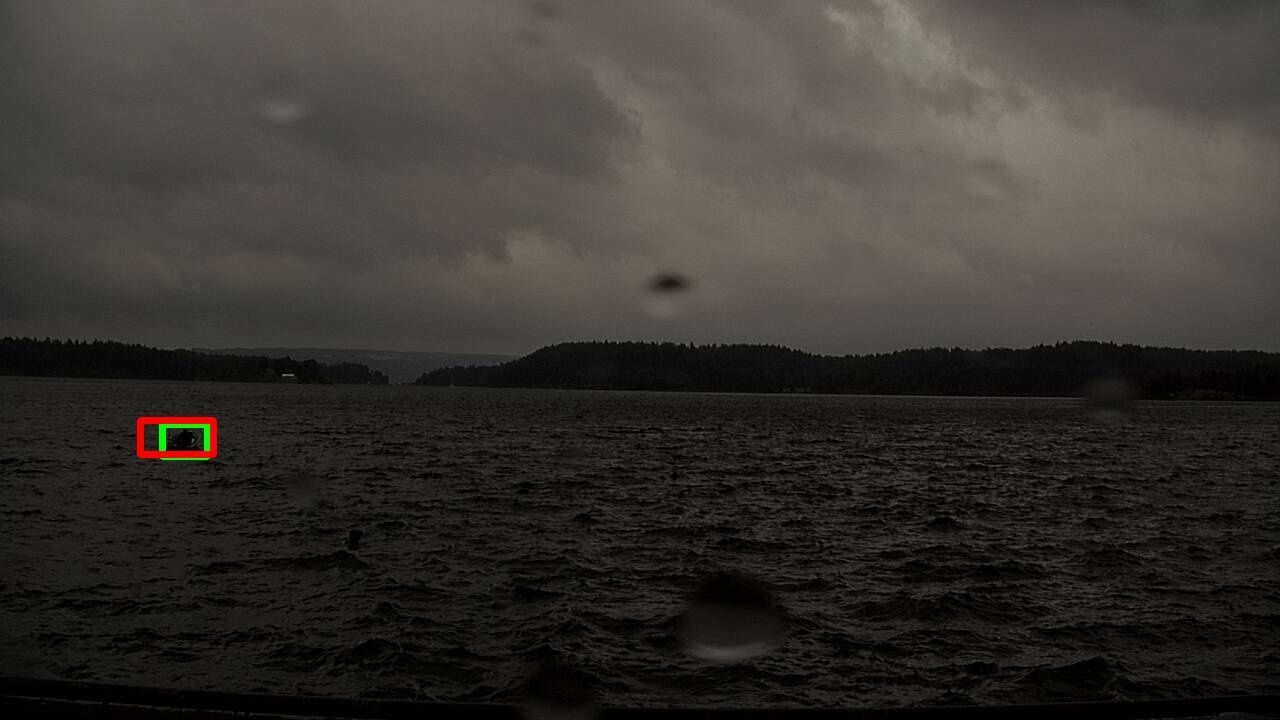
\includegraphics[width=.9\linewidth]{results/case_buildings/bigbox_bcbf/SSD3/selected_06_14_axis0049.jpg}
  \caption{SSD3}
  \label{fig:sfig2}
\end{subfigure}

\begin{subfigure}{.5\textwidth}
  \centering
  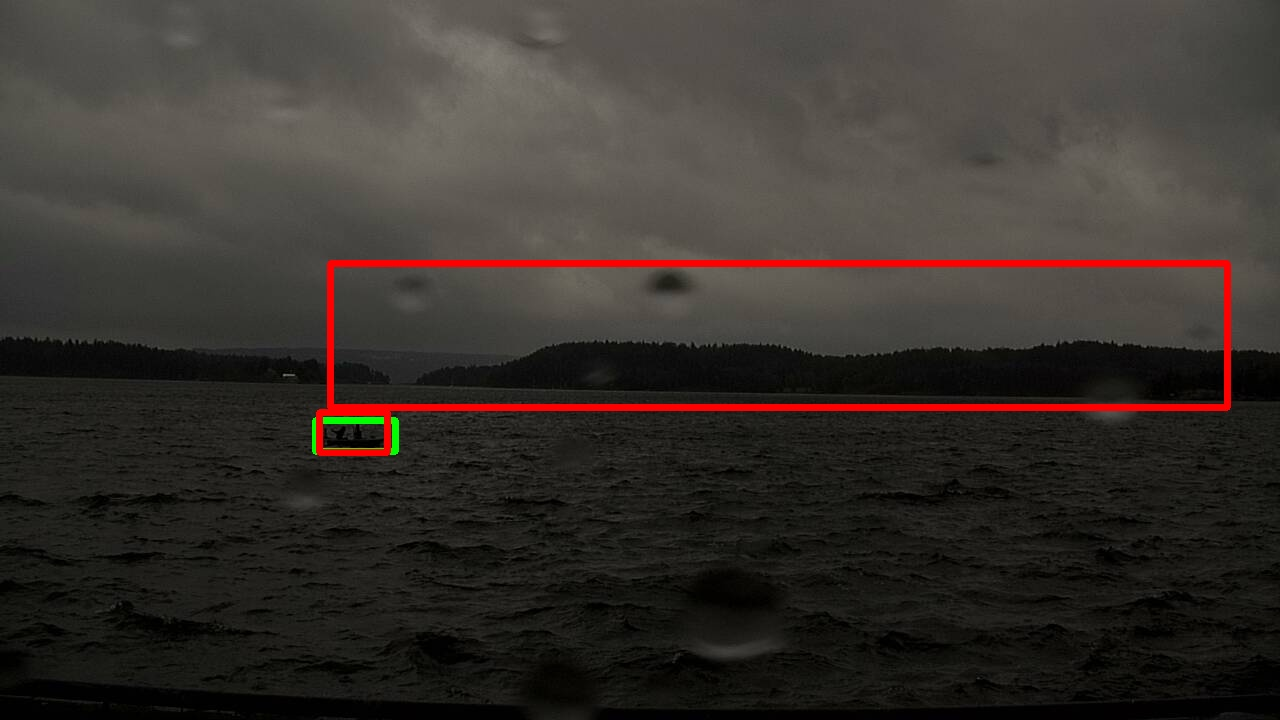
\includegraphics[width=0.9\linewidth]{results/case_buildings/bigbox_bcbf/SSD2/selected_06_14_axis0019.jpg}
  \caption{SSD2}
  \label{fig:sfig1}
\end{subfigure}%
\begin{subfigure}{.5\textwidth}
  \centering
  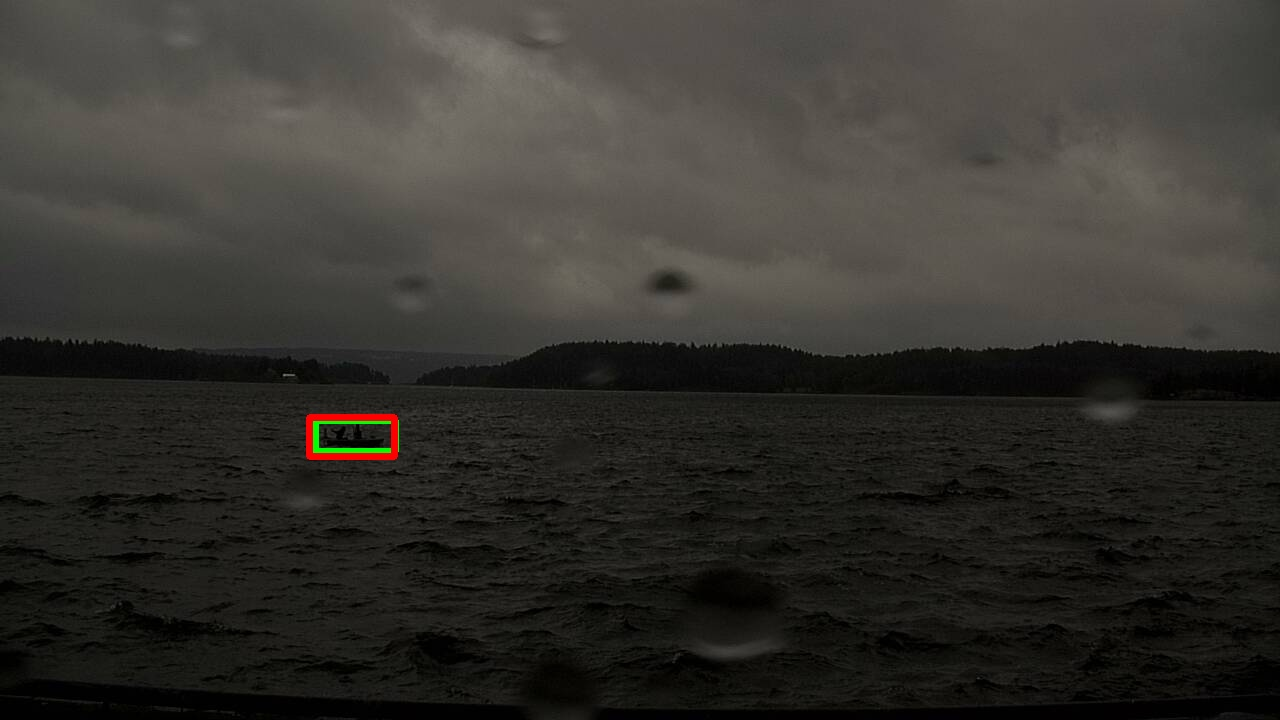
\includegraphics[width=.9\linewidth]{results/case_buildings/bigbox_bcbf/SSD3/selected_06_14_axis0019.jpg}
  \caption{SSD3}
  \label{fig:sfig2}
\end{subfigure}

\begin{subfigure}{.5\textwidth}
  \centering
  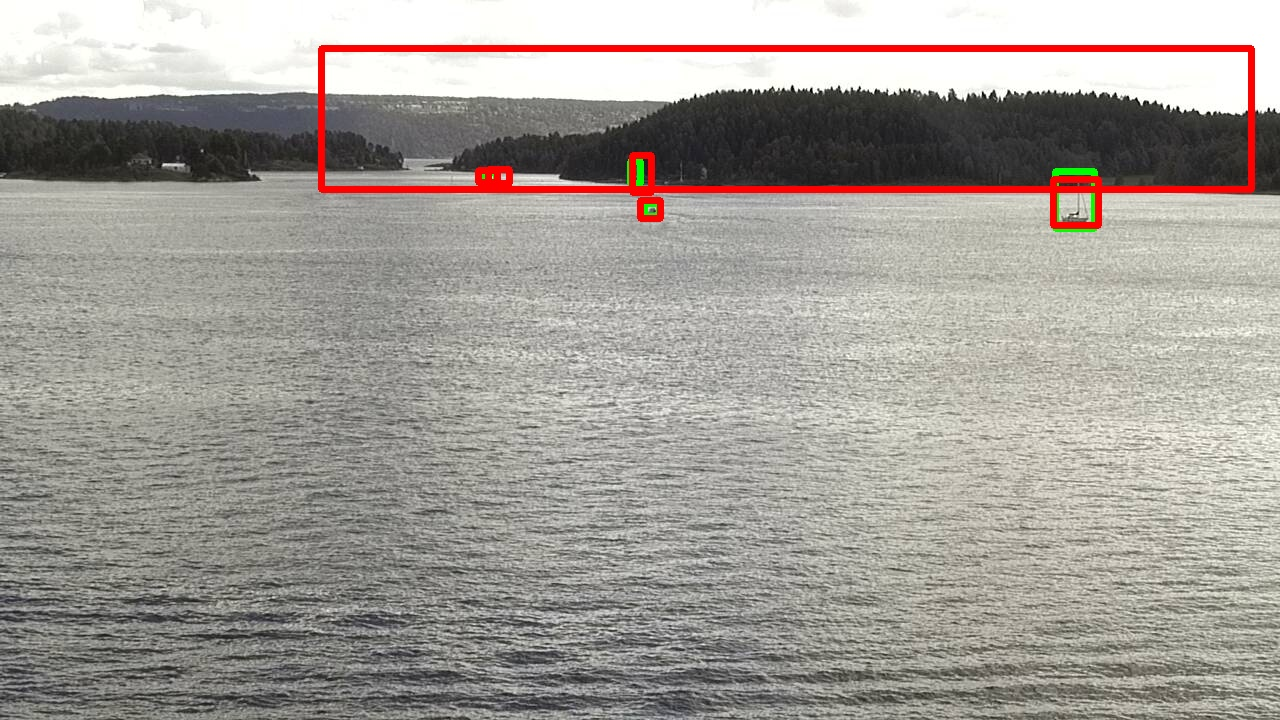
\includegraphics[width=0.9\linewidth]{results/case_buildings/bigbox_bcbf/SSD2/selected_08_04_frame3470.jpg}
  \caption{SSD2}
  \label{fig:sfig1}
\end{subfigure}%
\begin{subfigure}{.5\textwidth}
  \centering
  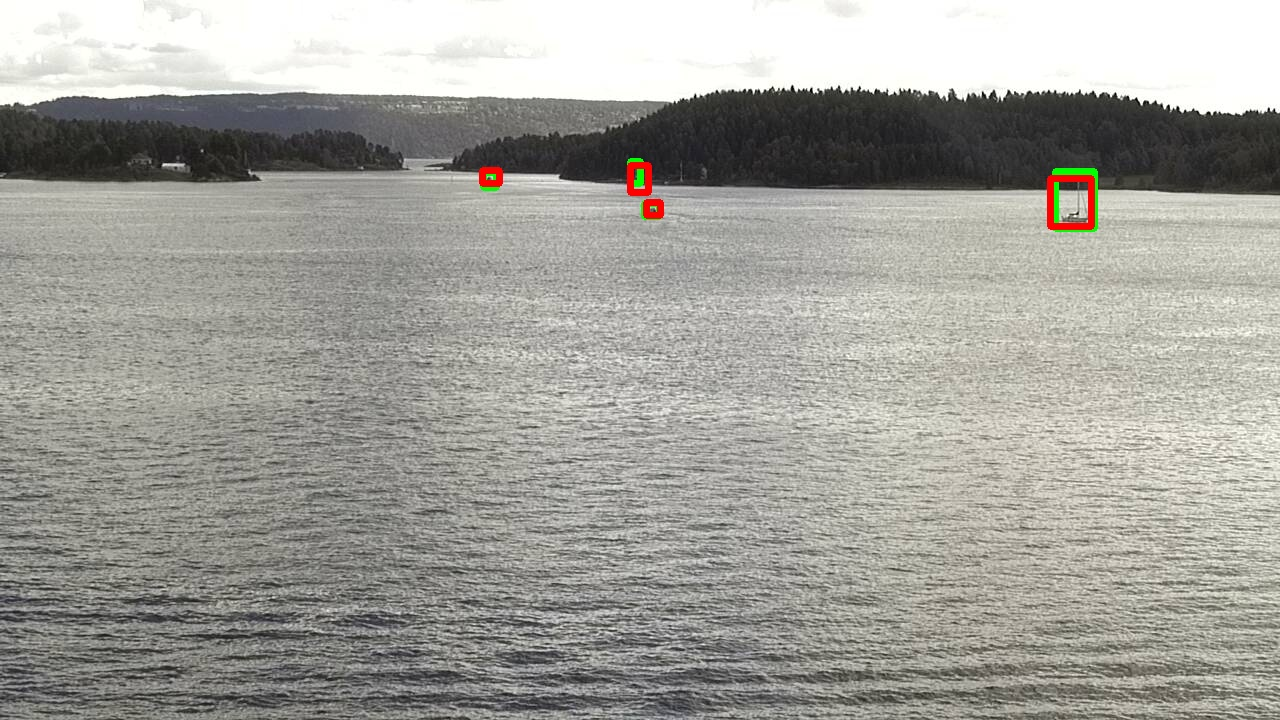
\includegraphics[width=.9\linewidth]{results/case_buildings/bigbox_bcbf/SSD3/selected_08_04_frame3470.jpg}
  \caption{SSD3}
  \label{fig:sfig2}
\end{subfigure}

\begin{subfigure}{.5\textwidth}
  \centering
  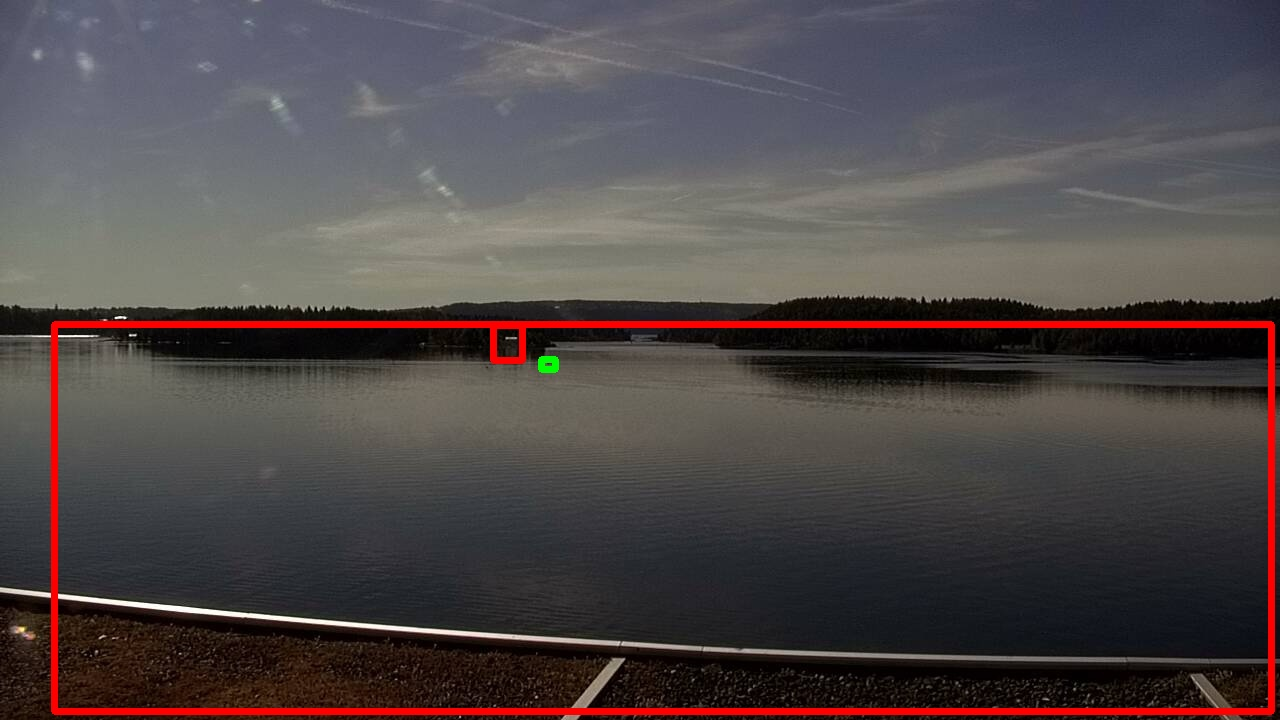
\includegraphics[width=0.9\linewidth]{results/case_buildings/bigbox_bcbf/SSD2/selected_08_07_frame0290.jpg}
  \caption{SSD2}
  \label{fig:sfig1}
\end{subfigure}%
\begin{subfigure}{.5\textwidth}
  \centering
  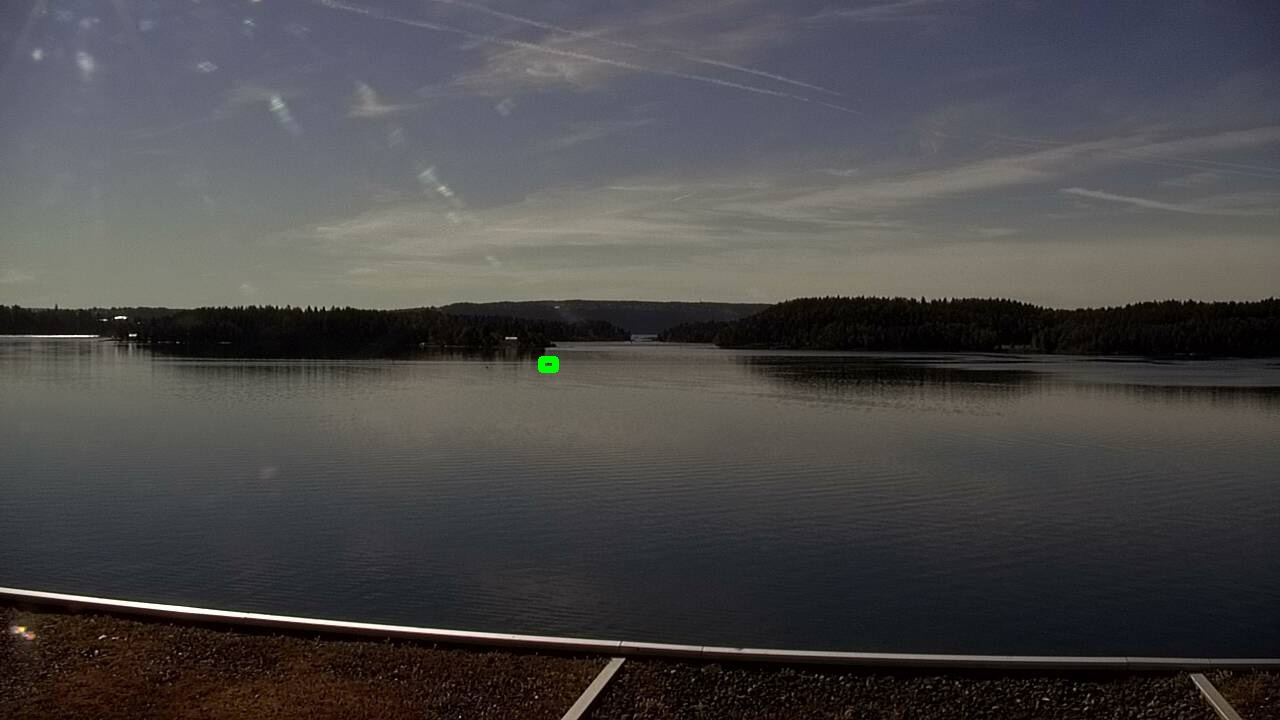
\includegraphics[width=.9\linewidth]{results/case_buildings/bigbox_bcbf/SSD3/selected_08_07_frame0290.jpg}
  \caption{SSD3}
  \label{fig:sfig2}
\end{subfigure}

\caption{plots of....}
\label{fig:fig}
\end{figure}

\begin{figure}
\begin{subfigure}{.5\textwidth}
  \centering
  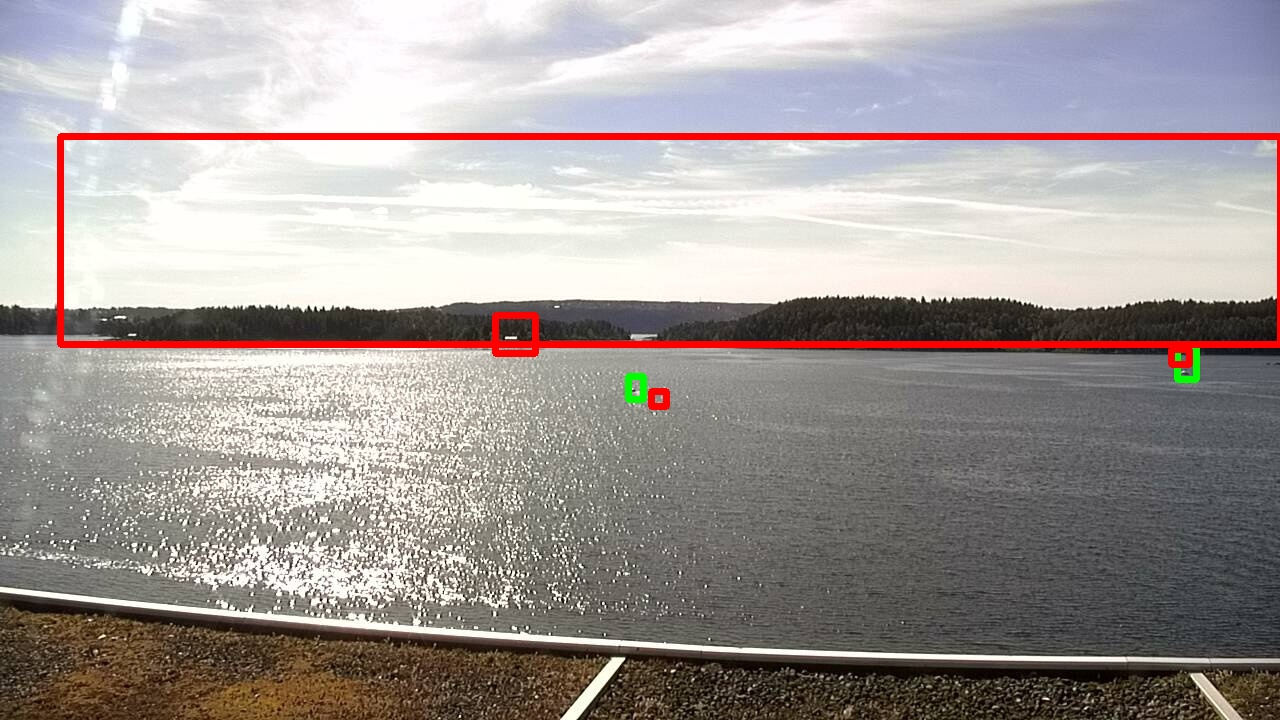
\includegraphics[width=0.9\linewidth]{results/case_buildings/bigbox_bcbf/SSD2/selected_08_07_frame1916.jpg}
  \caption{SSD2}
  \label{fig:sfig1}
\end{subfigure}%
\begin{subfigure}{.5\textwidth}
  \centering
  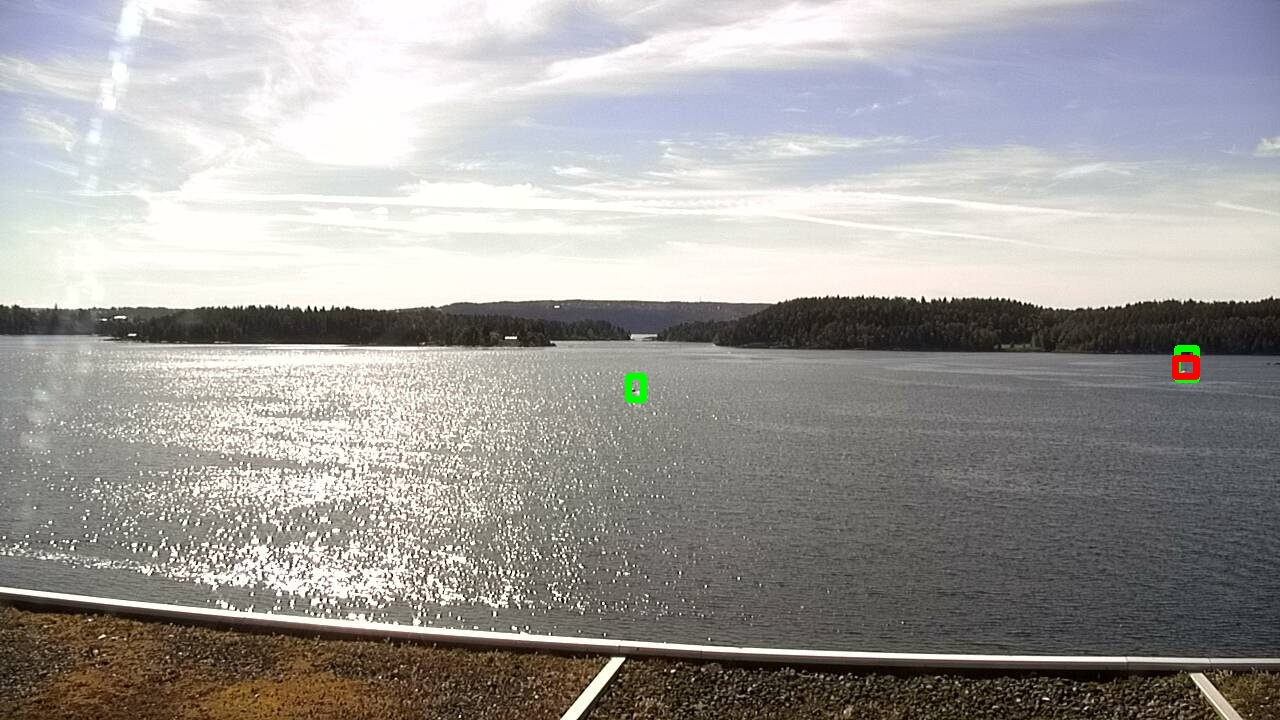
\includegraphics[width=.9\linewidth]{results/case_buildings/bigbox_bcbf/SSD3/selected_08_07_frame1916.jpg}
  \caption{SSD3}
  \label{fig:sfig2}
\end{subfigure}

\begin{subfigure}{.5\textwidth}
  \centering
  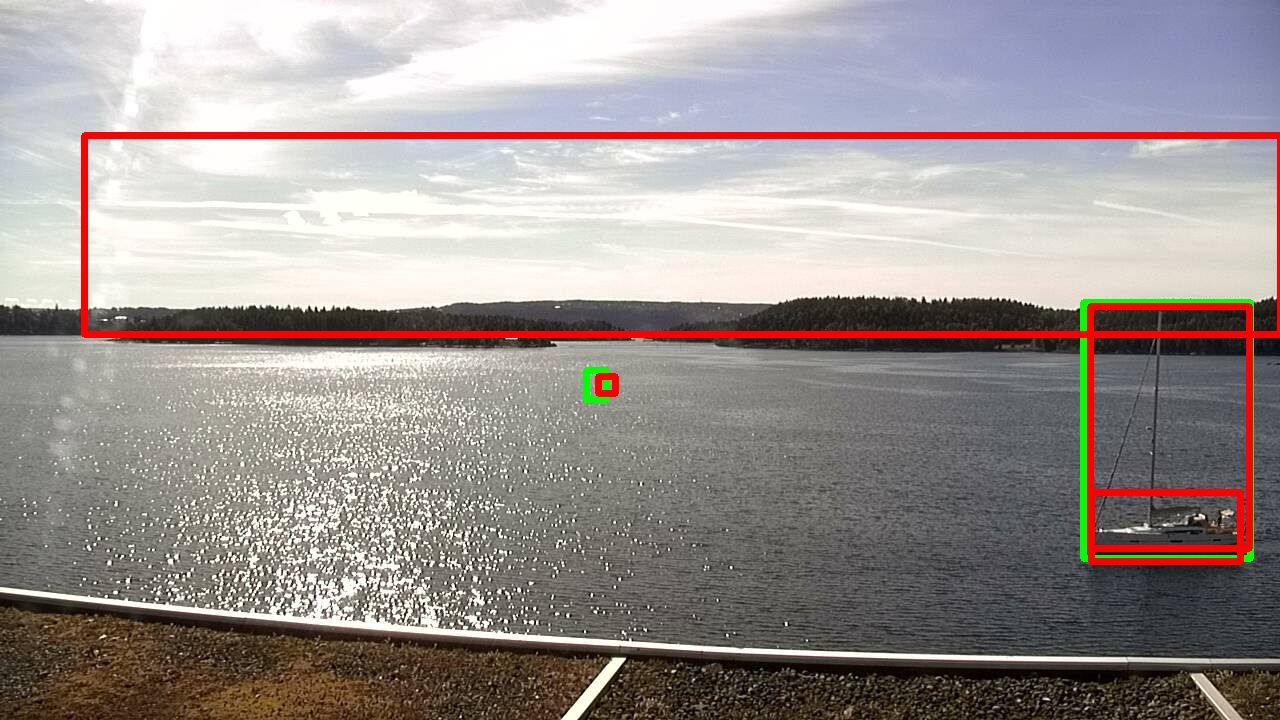
\includegraphics[width=0.9\linewidth]{results/case_buildings/bigbox_bcbf/SSD2/selected_08_07_frame2176.jpg}
  \caption{SSD2}
  \label{fig:sfig1}
\end{subfigure}%
\begin{subfigure}{.5\textwidth}
  \centering
  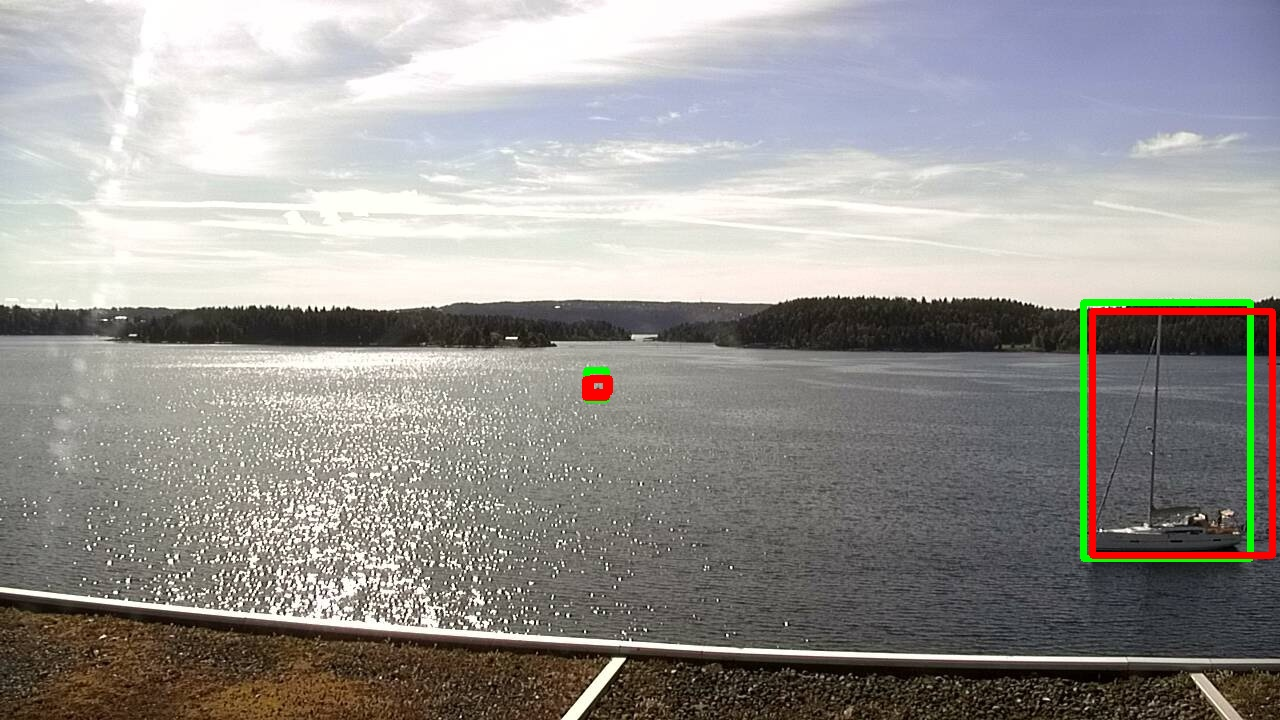
\includegraphics[width=.9\linewidth]{results/case_buildings/bigbox_bcbf/SSD3/selected_08_07_frame2176.jpg}
  \caption{SSD3}
  \label{fig:sfig2}
\end{subfigure}

\begin{subfigure}{.5\textwidth}
  \centering
  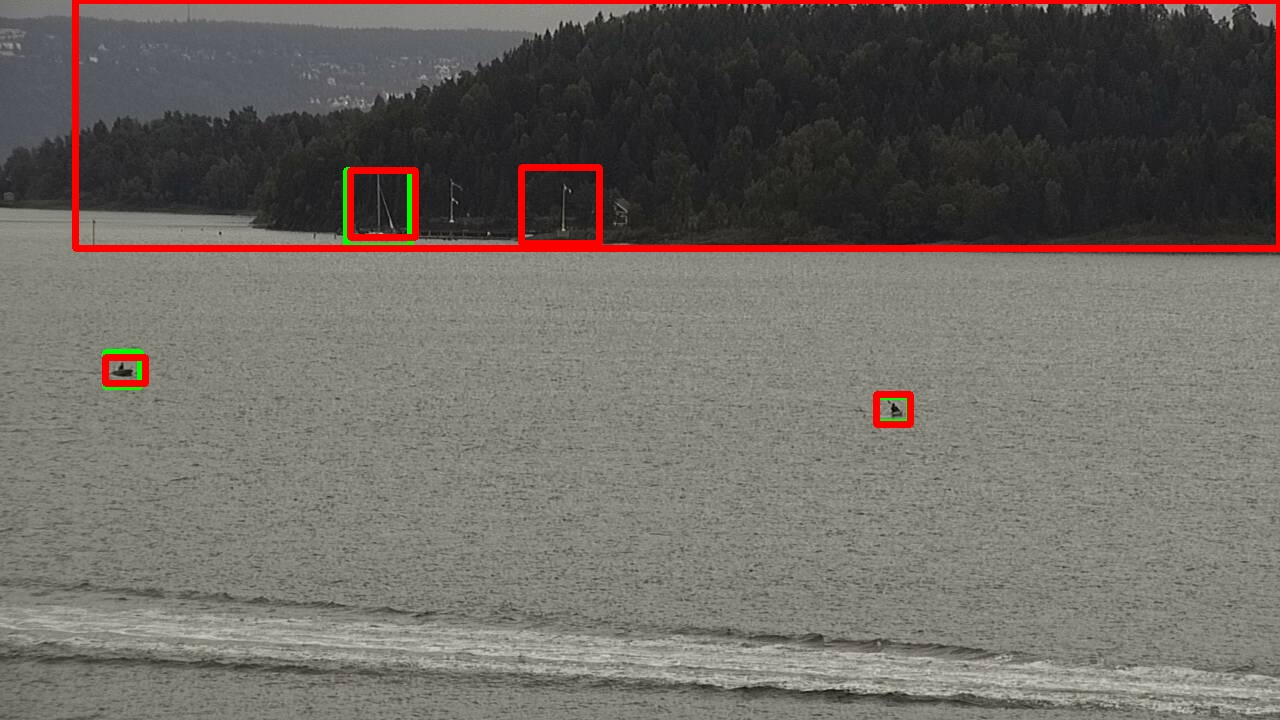
\includegraphics[width=0.9\linewidth]{results/case_buildings/bigbox_bcbf/SSD2/selected_08_09_frame4530.jpg}
  \caption{SSD2}
  \label{fig:sfig1}
\end{subfigure}%
\begin{subfigure}{.5\textwidth}
  \centering
  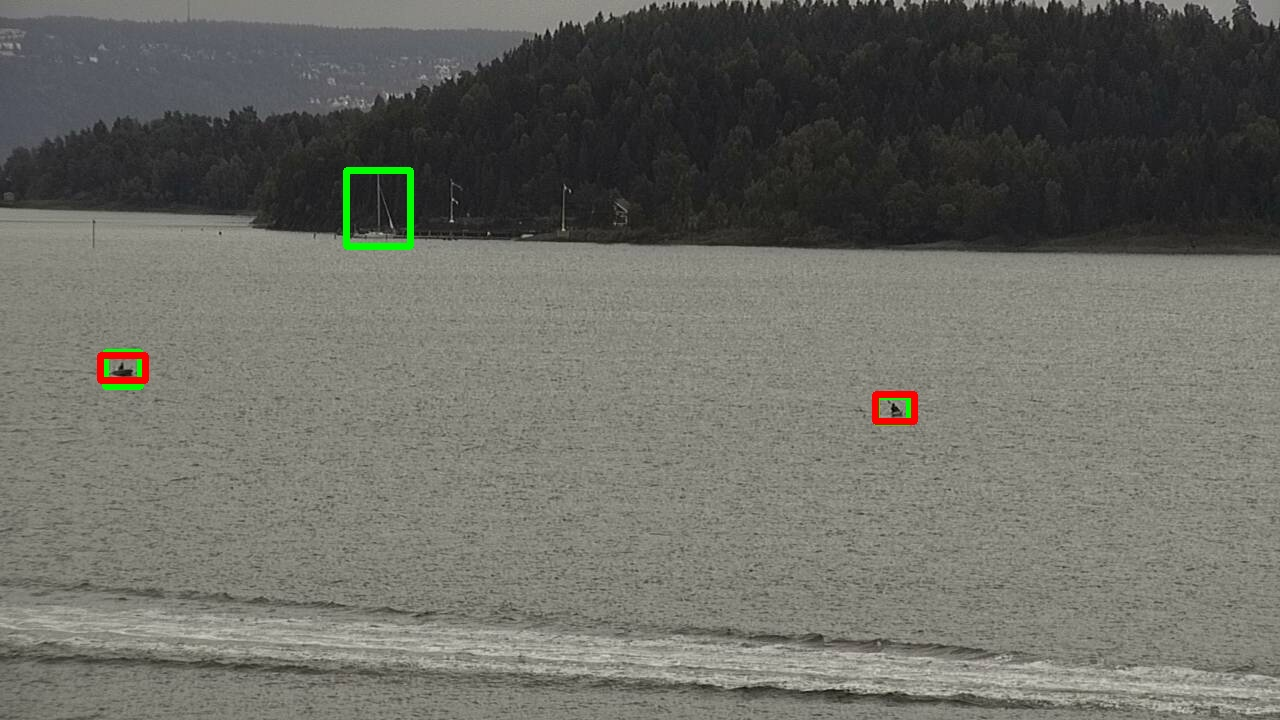
\includegraphics[width=.9\linewidth]{results/case_buildings/bigbox_bcbf/SSD3/selected_08_09_frame4530.jpg}
  \caption{SSD3}
  \label{fig:sfig2}
\end{subfigure}

\begin{subfigure}{.5\textwidth}
  \centering
  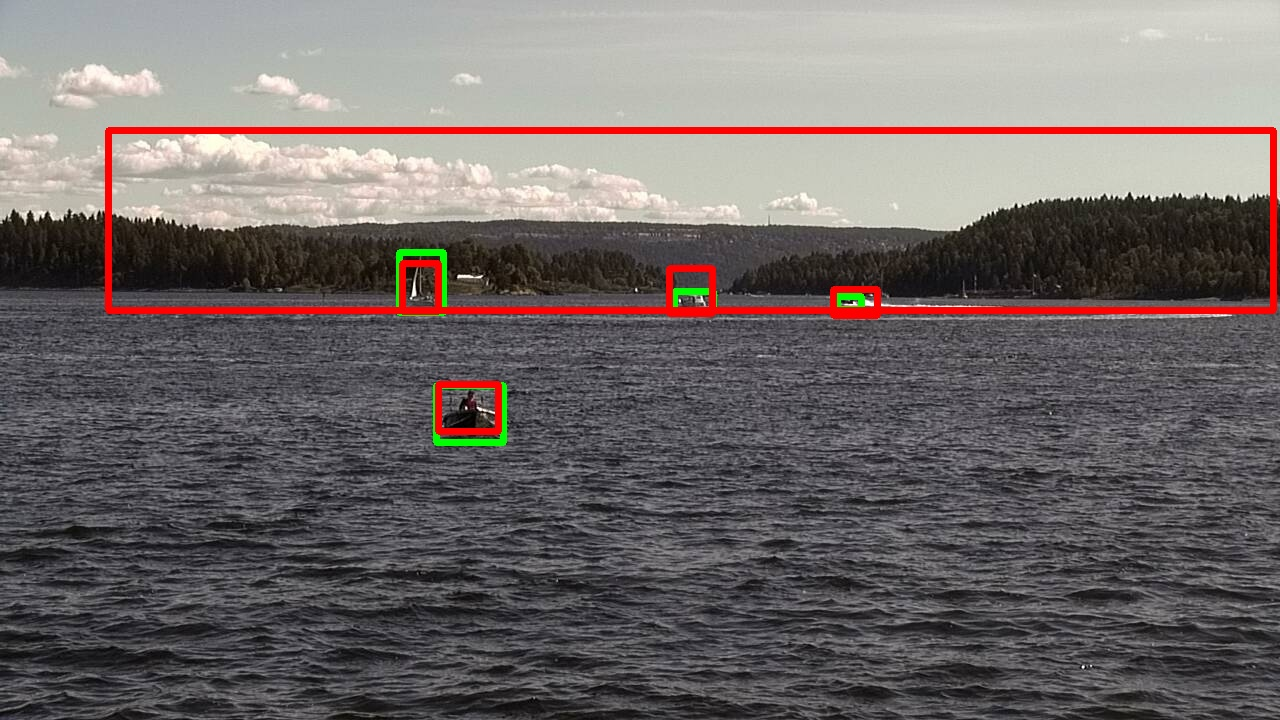
\includegraphics[width=0.9\linewidth]{results/case_buildings/bigbox_bcbf/SSD2/selected_08_14_frame1150.jpg}
  \caption{SSD2}
  \label{fig:sfig1}
\end{subfigure}%
\begin{subfigure}{.5\textwidth}
  \centering
  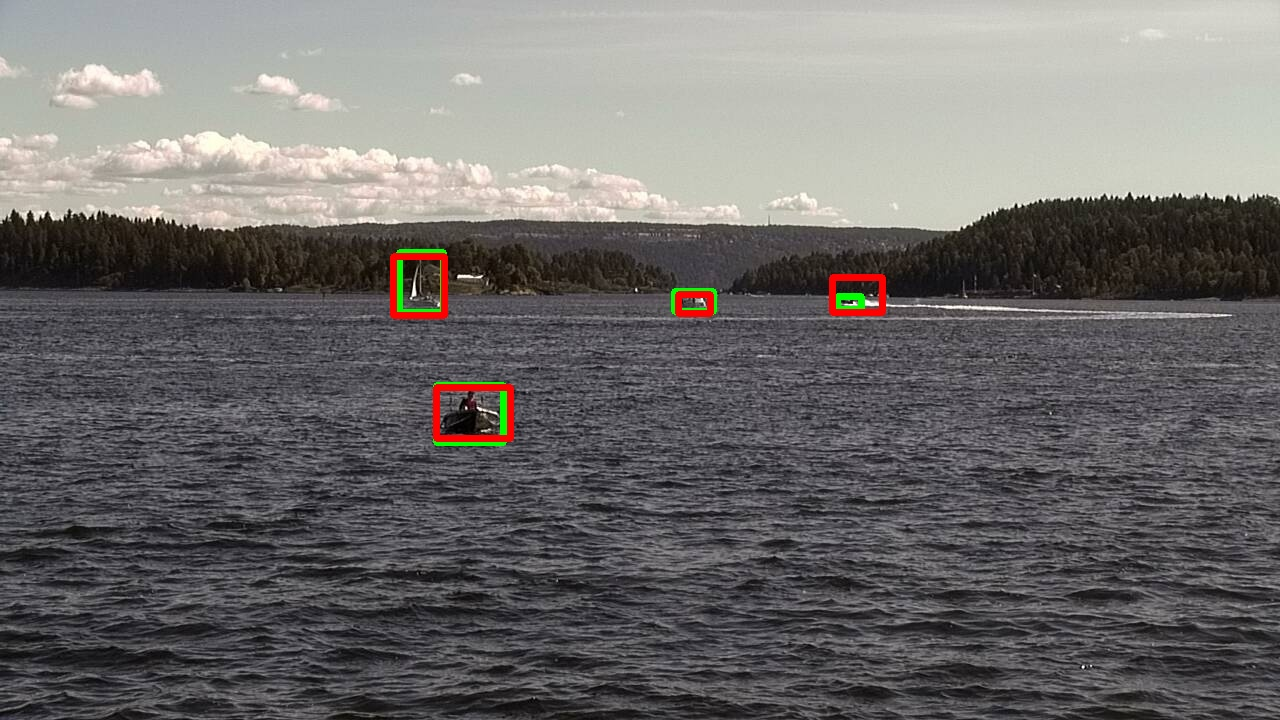
\includegraphics[width=.9\linewidth]{results/case_buildings/bigbox_bcbf/SSD3/selected_08_14_frame1150.jpg}
  \caption{SSD3}
  \label{fig:sfig2}
\end{subfigure}

\caption{plots of....}
\label{fig:fig}
\end{figure}

\section{Yolo2 and Yolo3 on bc bf}

\subsection{Yolo2 better than Yolo3}
\subsection{Yolo3 better than Yolo2}
\subsection{Same misclassifications}
